\subsection{Data Types}
\label{sec:data_types}

The \sunpypkg package provides two core data types that are designed to provide a general, standard, and consistent interface for loading and representing solar data across different instruments and missions.
The core data types currently provided in \sunpypkg are \Timeseries and \Map, which support 1D temporal data and 2D image data, respectively. 
The purpose of these core classes is to accommodate the user with a standard data structure regardless of the data source (i.e. observational data from separate instruments). 
They maintain a consistent interface for accessing solar data attributes such as the data array itself as well as the metadata and relevant units. 
This allows for an easier workflow in the analysis of solar data observations.
These core classes also include functionality for data manipulation and data visualization. 
This section provides an overview of the \Timeseries and \Map data types.

\subsubsection{\Timeseries}
\label{sec:timeseries}
Many observations in the field of solar physics consist of time series data. 
For example, the X-ray Sensor aboard the Geostationary Operational Environmental Satellite (GOES), which is used as the classification standard for solar flares, continuously measures the disk-integrated X-ray flux as a function of time in two broadband channels. 
The \Timeseries class in \sunpypkg aims to accommodate the necessary requirements to represent solar time series data.

\Timeseries allows users to load time series data from a variety of solar instruments and contain the data with appropriate units and time scales (see \autoref{sec:units}). 
 A user can create a \Timeseries either from data files stored locally (i.e. observational datasets acquired through \Fido (see \autoref{sec:fido}), or manually from custom time series data. 
 The data array as well as the metadata and units data are stored as attributes to the \Timeseries class. 

A large amount of functionality exists within \Timeseries for the manipulation of solar time series data.
This includes the ability to add, update, truncate, re-sample and combine data within a \Timeseries or combine multiple \Timeseries together. 
\Timeseries also has built-in visualization methods to allow for easy inspection. 
An example of a \Timeseries created from GOES X-ray sensor observations during a day for which a solar flare is present is shown in Figure~\ref{fig:timeseries_example}.

\begin{figure}
    \centering
    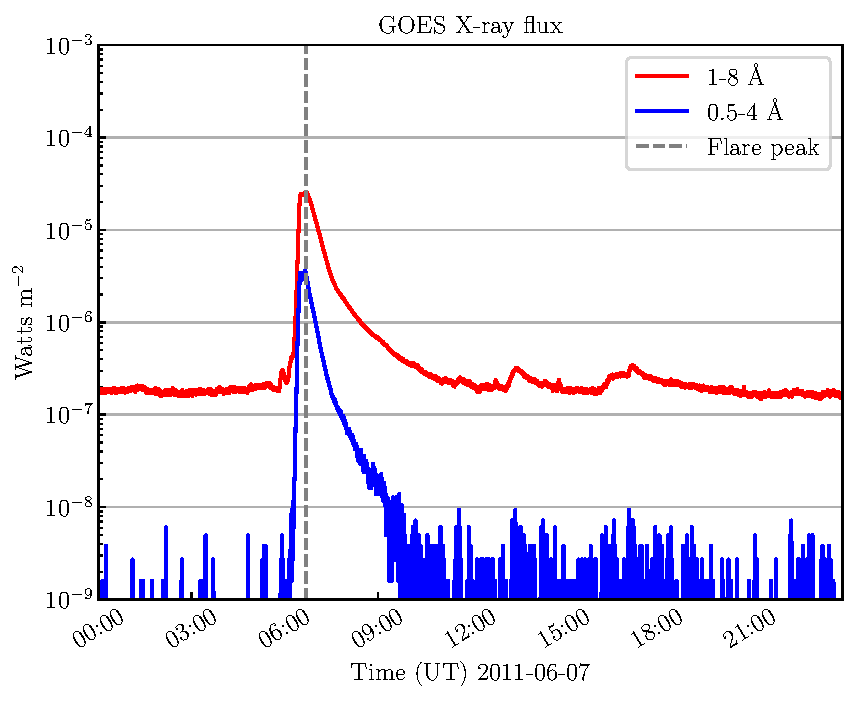
\includegraphics[width=0.55\textwidth]{figures/timeseries_example.pdf}
    \caption{An example of a GOES X-ray Sensor \Timeseries plotted over a 24 hour period. The two colors time series represent the two broadband channels of GOES 1--8~\AA\ (red) and 0.5--4~\AA\ (blue).  A solar flare is noted by the increase in flux and the grey dashed line denotes the flare peak as found from the Helio Event Knowledgebase (HEK).}
    \label{fig:timeseries_example}
\end{figure}

\Timeseries currently supports the data sources listed in Table \ref{tab:instruments} in addition to indices from the National Oceanic and Atmospheric (NOAA) Space Weather Prediction Center (SWPC) that track the solar cycle and its predicted progression. Due to its flexible data structure, it is easy to add additional instruments and data sources to the \Timeseries object.

%%%%%%%%%%%%%%%% TABLE %%%%%%%%%%%%%%%%%%%
\begin{table}
\begin{center}
\begin{tabular}{|p{12cm}|c|c|}
\hline
& \\
\textbf{Supported by \Timeseries}& \textbf{Instrument reference}\\
\hline
\hline
\textit{Geostationary Operational Environmental Satellite (GOES)} X-ray Sensor (XRS) & \citet{garcia94, hanser96} \\
\hline
\textit{Fermi} Gamma-ray Burst Monitor (GBM) &  \citet{meegan2009fermi} \\
\hline
\textit{Nobeyama Radioheliograph (NoRH)} & \citet{nakajima1994nobeyama} \\
\hline
\textit{PRoject for Onboard Autonomy (PROBA2)} Large Yield Radiometer (LYRA) & \citet{dominique2013lyra} \\
\hline
\textit{Solar Dynamics Observatory (SDO)} EUV Variability Experiment (EVE) & \citet{woods2010extreme}  \\
\hline
\textit{Reuven Ramaty High Energy Solar Spectroscopic Imager (RHESSI)} & \citet{lin2003reuven} \\
\hline
 & \\
\textbf{Supported by \Map} & \textbf{Instrument reference} \\
\hline
\hline
\textit{COronal Solar Magnetism Observatory (COSMO)} K-coronagraph (K-Cor) & \citet{dewijn12} \\
\hline
\textit{Hinode} X-Ray Telescope (XRT) & \citet{golub2008x}  \\
\hline
\textit{Interface Region Imaging Spectrograph (IRIS)} Slit Jaw Imager (SJI) & \citet{DePontieu2014}  \\
\hline
\textit{PRoject for Onboard Autonomy (PROBA2)} Sun Watcher using Active Pixel System detector and Image Processing (SWAP) & \citet{seaton2013swap} \\
\hline
\textit{Reuven Ramaty High Energy Solar Spectroscopic Imager (RHESSI)} & \citet{lin2003reuven} \\
\hline
\textit{Solar and Heliospheric Observatory (SOHO)} Extreme ultraviolet Imaging Telescope (EIT) & \citet{delaboudiniere1995eit}\\
\hline
\textit{Solar and Heliospheric Observatory (SOHO)} Large Angle Spectroscopic COronagraph (LASCO) & \citet{brueckner1995large} \\
\hline
\textit{Solar and Heliospheric Observatory (SOHO)} Michelson Doppler Imager (MDI) & \citet{scherrer1995solar}\\
\hline
\textit{Solar Dynamics Observatory (SDO)} Atmospheric Imaging Assembly (AIA) & \citet{lemen2012} \\
\hline
\textit{Solar Dynamics Observatory (SDO)} Helioseismic and Magnetic Imager (HMI) & \citet{schou12}  \\
\hline
\textit{Solar TErrestrial RElations Observatory (STEREO)} Extreme Ultraviolet Imager (EUVI), COronagraph 1 and 2 (COR1/2) for both \textit{STEREO} A and B & \citet{howard2008sun} \\
\hline
\textit{Transition Region and Coronal Explorer (TRACE)}  & \citet{handy99}  \\
\hline
\textit{Yohkoh} Soft X-ray Telescope (SXT) & \citet{tsuneta1991soft}  \\
\hline
\end{tabular}
\end{center}
\caption{The following table outlines the instruments supported by the \Timeseries and \Map objects described in Section \ref{sec:data_types}.}
\label{tab:instruments}
\end{table}
%%%%%%%%%%%%%%%% TABLE %%%%%%%%%%%%%%%%%%%

\subsubsection{\Map}
\label{sec:map}
2D images are another commonly-used data format in solar physics. 
For example, the Helioseismic and Magnetic Imager (HMI) instrument aboard the Solar Dynamics Observatory (SDO) maps the magnetic field at the solar photosphere across the entire solar disk every 45 seconds with 4k $\times$ 4k pixel resolution.
Data in this form exists for multiple wavelengths from a wide range of both space- and ground- based instruments.
These high resolution image sets require precise coordinate information in order to undertake scientific studies, particularly when performing multi-instrument observations. 

The \Map class in \sunpypkg provides a framework to contain and analyze 2D image data that have an associated coordinate frame. 
A \Map can be created by providing input data files located locally or fetched via the \sunpypkg data search and retrieval interface \Fido (see \autoref{sec:fido}).
The \Map class will automatically detect the instrument of the input data files and subsequently search the specific metadata to infer the coordinate system from the appropriate FITS keywords \citep{refId0, 2006A&A...449..791T}.
Other source-specific metadata is also loaded into the \Map class such as color tables and appropriate image scaling for each instrument.
It is also possible to create a custom \Map from both a 2D data array and the appropriate metadata, such as coordinate information.

The \Map class contains the image data array, coordinate information and relevant metadata as attributes, all of which can be easily accessed by the user. 
Visualization methods are also provided by \Map to inspect and plot solar image data. 
This includes the ability for \Map to plot the image data in a way that represents the world coordinates of the image accurately (see \autoref{sec:coords} for more on solar coordinates).
This allows the user to plot coordinates of interest on a \Map while correctly accounting for the coordinate frame. 
Other plotting components in \Map include the ability to mask and clip the image data. 

An example of a \Map using data from the Atmospheric Imaging Assembly (AIA) aboard the \textit{Solar Dynamics Observatory (SDO)} is shown in \autoref{fig:map_example}. 
This plot demonstrates the plotting and manipulation ability of \Map.
The left panel shows the full disk image of the Sun with the relevant image color table and scaling for the observation, and the right panel shows a cropped image in the field of view of the white box in the left panel, highlighting a solar flare of interest.

The \Map class also provides functionality to analyze multiple images, such as overlaying images from different instruments with overlapping fields of view, or to combine multiple images together in a time-ordered sequence.  
This includes the ability to co-align images from different instruments or images taken at different times, which is particularly useful to users performing multi-instrument studies. 


\begin{figure}
    \centering
    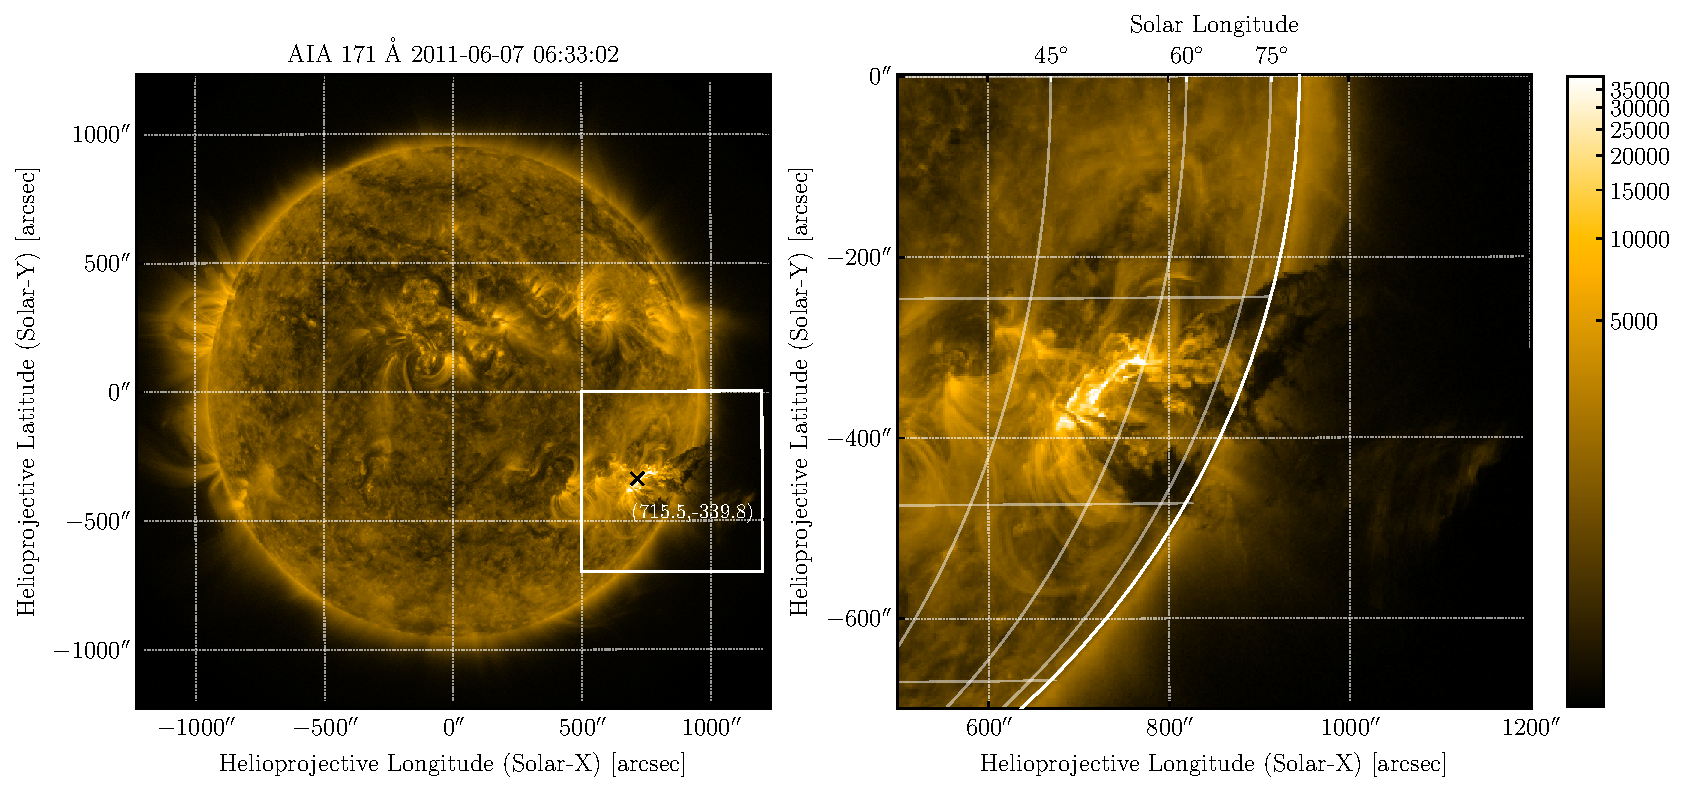
\includegraphics[width=0.97\textwidth]{figures/map_example.pdf}
    \caption{An example of a \sunpypkg \Map plotted from observations of the 171~\AA\ wavelength channel of the Atmospheric Imaging Assembly (AIA) aboard the Solar Dynamics Observatory (SDO).The left hand panel shows a full disk image of the Sun whereas the right hand panel shows a zoom in of the white box in the left hand panel, focusing on the flare that erupted (the same event as the \Timeseries plot in Figure~\ref{fig:timeseries_example}).}
    \label{fig:map_example}
\end{figure}

\Map currently supports the data sources listed in Table \ref{tab:instruments} as well as the Helioviewer JPEG2000 image files of for each of these data sources. Similar to \Timeseries, it is easy to add additional instruments and data sources to \Map. 
